\section{Berechnung dynamischer Nash-Flüsse mit schmalen Flüssen}\label{sec-nash-flow-extension}
In diesem Abschnitt soll es nun schließlich darum gehen, den Zusammenhang zwischen dynamischen Nash-Flüssen und schmalen Flüssen mit Zurücksetzen aufzuzeigen.
Danach wird kurz auf die Existenz dynamischer Nash-Flüsse und deren Berechnung bei konstanter Einflussrate in das Netzwerk eingegangen.
Dazu wird wieder die Notation dynamischer Flüsse aus den Kapiteln~\ref{chapter-dynamic-flows} und~\ref{chapter-nash-flows} verwendet.

Für diese Ergebnisse werden schmale Flüsse mit einer kleinen Modifikation verwendet:

\begin{definition}[Normierter schmaler Fluss]\label{def-normalized-thin-flow}
	Seien ein $s$-Netzwerk $\mathcal{N}$ und ein $b$-Fluss $f$ gegeben.
	Für einen $s$-$v$-Pfad $P=(e_1, \dots, e_k)$ bezeichnet die \emph{normierte Auslastung von $P$} die Verkettung $\rho_{e_k}(\cdot, f_{e_k}) \circ \cdots \circ \rho_{e_1}(\cdot, f_{e_1})(1)$.
	Die zu $f$ gehörige \emph{normierte Knotenauslastung} $l\in\R^V$ ist für jeden Knoten $v\in V$ die minimale Auslastung eines $s$-$v$-Pfades.
	Dann heißt $f$ ein \emph{normierter $b_s$-wertiger schmaler Fluss mit Zurücksetzen auf $E_1$}, falls die Auslastung jedes $s$-$v$-Pfades mit positivem Fluss $l_v$ beträgt.
\end{definition}

Schnell kann man sehen, dass sich die Ergebnisse aus den vorherigen Kapiteln ohne großen Aufwand übertragen lassen:

\begin{proposition}
	Es sei ein $b$-Fluss $f$ in einem $s$-Netzwerk $\mathcal{N}$ mit $b_s > 0$ gegeben.
	Man erhalte das Netzwerk $\mathcal{N}'$ aus $\mathcal{N}$, indem man einen zusätzlichen Knoten $s'$ und eine Kante $(s, s')$ mit Kapazität $b_s$ hinzufügt und das Angebot von $s$ mit $b'_s \coloneq 0$ und $b'_{s'}\coloneq b_s$ auf $s'$ überträgt.
	Ergänzt man $f$ durch den Flusswert $b_s$ auf der Kante $(s', s)$, so erhält man den $b'$-Fluss $f'$.
	
	Dann ist die normierte Auslastung jedes $s$-$v$-Pfads $P$ in $\mathcal{N}$ gerade die Auslastung des $s'$-$v$-Pfads $P'$ in $\mathcal{N}'$, der vor dem Pfad $P$ noch die Kante $(s', s)$ benutzt.
	Insbesondere ist $f$ genau dann ein normierte schmaler Fluss in $\mathcal{N}$, wenn $f'$ ein schmaler Fluss in $\mathcal{N'}$ ist.
\end{proposition}
\begin{proof}
	Die Kante $(s', s)$ hat für jeden $b'$-Fluss Auslastung $1$.
	Daher ist die normierte Auslastung eines $s$-$v$-Pfades gerade die Auslastung vom durch die Kante $(s', s)$ verlängerten Pfad.
\end{proof}

Dadurch können normierte schmale Flüsse durch die Bestimmung nicht-normier\-ter schmalen Flusses ermittelt werden.
Außerdem können Lemma~\ref{lemma-equivalent-thin-flow} ohne Verän\-derung und Lemma~\ref{lemma-thin-flow-t-def} mit der kleinen Modifikation, dass statt~\ref{def-thin-flow-source}, also $l_s = 0$, hier $l_s = 1$ gelten muss, für normierte schmale Flüsse übernommen werden.

Das folgende Theorem liefert das Resultat, dass ein dynamischer Nash-Fluss zu jedem Zeitpunkt $\theta\in\R$ einen normierten schmalen Fluss mit Zurücksetzen induziert.
Die Voraussetzung, dass hierbei die entsprechenden Ableitungen existieren, kann man dadurch rechtfertigen, dass nach \cite[Folgerung~4.12~b)]{Elstrodt2011Abs} absolut stetige Funktionen fast überall differenzierbar sind.
Zudem gilt nach \cite[Aufgabe~4.10]{Elstrodt2011Abs} die Substitutionsregel für absolut stetige Funktionen, wodurch
\[
\int_{l_v(\theta_1)}^{l_v(\theta_2)} f_{vw}^+(t) \diff t = \int_{\theta_1}^{\theta_2} f_{vw}^+(l_v(t)) l_v'(t) \diff t
\]
gefolgert werden kann.
Daher gilt auch für fast alle $\theta\in\R$:
\[ 
x_{vw}'(\theta) = f_{vw}^+(l_v(\theta))l_v'(\theta) \text{~~~ bzw. analog ~~~} x_{vw}'(\theta) = f_{vw}^-(l_w(\theta)) l_w'(\theta).
\]

\begin{theorem}
	Seien ein dynamischer Nash-Fluss $f$ im Graphen $(V,E)$ sowie ein Zeitpunkt $\theta\in\R$ gegeben.
	Existieren die Ableitungen $x_{vw}'(\theta)$ und $l_v'(\theta)$ mit 
	\[
	x_{vw}'(\theta) = f_{vw}^+(l_v(\theta)) l_v'(\theta)= f_{vw}^-(l_w(\theta))l_w'(\theta)
	\]
	für alle Kanten $vw$ und Knoten $v$, so ist der statische Fluss $x'(\theta) \in \R^{E_\theta}$, eingeschränkt auf die zu $\theta$ aktiven Kanten, ein normierter schmaler Fluss mit Zurück\-setzen auf den Kanten mit Warteschlange $E_1\coloneq \{vw\in E \mid q_{vw}(l_v(\theta))>0 \}$ von Wert $d(\theta)$.
	Dabei sind die Ableitungen $(l_v'(\theta))_{v\in V}$ die normierten Knotenauslastungen.
\end{theorem}
\begin{proof}
	Man bemerke zunächst $l_s'(\theta) = 1$.
	Da außerdem der Einfluss in das Netzwerk 
	\[
	d(\theta)= \sum_{e\in \delta^+(s)} f_e^+(\theta) - \sum_{e\in\delta^-(s)} f_e^-(\theta) = \sum_{e\in \delta^+(s)} x_e'(\theta) - \sum_{e\in\delta^-(s)} x_e'(\theta)
	\]
	erfüllt, ist $x'(\theta)$ ein $d(\theta)$-wertiger Fluss, weil $x_e'(\theta)$ nach Lemma~\ref{lemma-x-locally-constant} für inaktive Kanten $e$ verschwindet. Es bleibt also die Bedingungen~\ref{def-thin-flow-x-zero}-\ref{def-thin-flow-no-resetting-edge} zu zeigen.
	
	Um Bedingung~\ref{def-thin-flow-no-resetting-edge} zu zeigen,
	nehme man an, dass die Warteschlange jeder eingehenden Kante $vw$ eines Knotens $w$ zur Zeit $l_v(\theta)$ leer ist.
	Da für alle $n\in\N$ eine eingehende und zur Zeit $\theta_n \coloneq \theta + 1/n$ aktive Kante existiert, gibt es eine Kante $vw$ die zu unendlich vielen $\theta_n$ aktiv ist.
	Betrachtet man diese Teilfolge $(\theta_{n_k})_{k\in\N}$ der aktiven Zeitpunkte von $vw$, ist $vw$ wegen der Stetigkeit auch zur Zeit $\theta$ aktiv und es gilt 
	\[
	l_w'(\theta) = \lim_{k\to\infty} \frac{l_w(\theta_{n_k})- l_w(\theta)}{1/n_k} = \lim_{k\to\infty} \frac{ l_v(\theta_{n_k}) + q_{vw}(l_v(\theta_{n_k})) - l_v(\theta) }{1/n_k} \geq l_v'(\theta).
	\]
	Also ist insbesondere $l_w'(\theta) \geq \min_{vw\in \delta^-(w)\cap E_\theta} l_v'(\theta)$.
	
	Sei nun eine Kante $vw\in E_\theta$, also eine aktive Kante zum Zeitpunkt $\theta$, gegeben. Man prüfe die Bedingungen~\ref{def-thin-flow-x-zero}, \ref{def-thin-flow-x-positive} und \ref{def-thin-flow-resetting-edge} jeweils in den folgenden drei Fällen:
	
	\begin{description}[leftmargin=0cm, topsep=0cm, itemindent=0.5cm]
		\item[1. Fall:] $\exists \varepsilon > 0:\forall \theta'\in (\theta, \theta + \varepsilon ] : q_{vw}(l_v(\theta')) > 0$.
		
		Nach Lemma~\ref{lemma-nash-flow-waiting-queue-implies-active-edge} ist $[\theta,\theta+\varepsilon]\subseteq \Theta_{vw}$.
		Außerdem ist $q_{vw}$ nach Proposition~\ref{prop-feasible-flow}~\ref{prop-feasible-flow-positive-queue} auf dem Intervall $[ l_v(\theta') , l_w(\theta') - \tau_{vw} )$ positiv, also insbesondere auf $( l_w(\theta)-\tau_{vw} , l_w(\theta + \varepsilon) - \tau_{vw} )$.
		Man folgere $x_{vw}(\theta + \varepsilon) - x_{vw}(\theta) = \int_{l_w(\theta)-\tau_{vw}}^{l_w(\theta + \varepsilon)-\tau_{vw}} f_{vw}^-(t+\tau_{vw}) dt
		= u_{vw} (l_w(\theta + \varepsilon) - l_w(\theta))$ mit~\ref{def-feasible-flow-queue-with-capacity}.
		Teilt man diese Gleichung durch $\varepsilon$, so erhält man für $\varepsilon\rightarrow 0$ die Bedingung $x_{vw}'(\theta) = u_{vw} l_w'(\theta)$.
		Ist $vw\in E_1$, so ist also Bedingung~\ref{def-thin-flow-resetting-edge} erfüllt.
		Für Bedingung~\ref{def-thin-flow-x-zero} setze man $x_{vw}'(\theta)=0$ voraus, wodurch $l_w'(\theta)=0$ folgt und mit der Monotonie von $l_v$ gilt $0 \leq l_v'(\theta)$.
		
		Ist $vw\notin E_1$, ist also die Warteschlange zum Zeitpunkt $l_v(\theta)$ leer, so gilt: $l_w(\theta+\varepsilon) - l_w(\theta) = l_v(\theta + \varepsilon) + q_{vw}(l_v(\theta + \varepsilon)) - l_v(\theta) \geq l_v(\theta + \varepsilon) - l_v(\theta)$.
		Teilt man wieder durch $\varepsilon$, so erhält man für $\varepsilon \rightarrow 0$ Bedingung~\ref{def-thin-flow-x-positive} mit $l_w'(\theta) \leq l_v'(\theta)$ und dem Resultat des letzten Absatzes.
		
		\item[2. Fall:] $\exists \varepsilon > 0: (\theta, \theta + \varepsilon] \subseteq \Theta_{vw}^c$.
		
		Nach Lemma~\ref{lemma-nash-flow-waiting-queue-implies-active-edge} gilt bereits $vw\notin E_1$ und nach Lemma~\ref{lemma-x-locally-constant} ist $x_{vw}'(\theta) = 0$. 
		Es muss also nur Bedingung~\ref{def-thin-flow-x-zero} geprüft werden:
		Wegen $\theta\in\Theta_{vw}$ gilt $l_w(\theta + \varepsilon) - l_w(\theta) < l_v(\theta + \varepsilon) - l_v(\theta)$.
		Teilt man diese Ungleichung durch $\varepsilon$, so erhält man für $\varepsilon\rightarrow 0$ die Bedingung $l_w'(\theta)\leq l_v'(\theta)$.
		
		\item[3. Fall:] $\forall \varepsilon>0: \exists \theta_{\varepsilon}\in (\theta, \theta+\varepsilon]: T_{vw}(l_v(\theta_\varepsilon)) = l_w(\theta_\varepsilon)$.
		
		Dies ist die exakte Umkehrung der Bedingung von Fall 2.
		Zusätzlich betrachte man diesen Fall nur, falls Fall 1 nicht eintritt.
		Das heißt, für alle $\theta_\varepsilon$ existiert ein $\theta'\in(\theta, \theta_\varepsilon]$ mit $q_{vw}(l_v(\theta')) = 0$; insbesondere ist $vw$ nicht in $E_1$ enthalten.
		Man wähle $\theta'_\varepsilon\coloneq \max\{ \theta'\in (\theta, \theta_\varepsilon] \mid q_{vw}(l_v(\theta')) = 0 \}$ als das Maximum solcher Zeitpunkte, welches aufgrund der Stetigkeit von $q_{vw}\circ l_u$ existiert.
		Nach Konstruktion ist $q_{vw}\circ l_v$ im Intervall $(\theta_\varepsilon', \theta_\varepsilon)$ positiv und nach Lemma~\ref{lemma-nash-flow-waiting-queue-implies-active-edge} ist die Kante $vw$ in diesem Intervall aktiv.
		Nun impliziert $\theta_\varepsilon'\in \Theta_{vw}$ gerade $\theta_\varepsilon\in\Theta_{vw}$, da $\Theta_{vw}$ ab\-ge\-schlossen ist.
		Daher folgt aus $l_w(\theta_\varepsilon') - l_w(\theta) = l_v(\theta_\varepsilon') - l_v(\theta)$ 		Bedingung~\ref{def-thin-flow-x-zero}, indem man durch $\theta_\varepsilon'-\theta$ teilt und $l_w'(\theta) = l_v'(\theta)$ für $\varepsilon\rightarrow0$ erhält.
		
		Für Bedingung~\ref{def-thin-flow-x-positive} bleibt zu zeigen, dass $x_{vw}'(\theta) /u_{vw}\leq l_w'(\theta)$ gilt.
		Wegen Bedingung~\ref{def-feasible-flow-capacity} ist $x_{vw}(\theta + \varepsilon)-x_{vw}(\theta) = \int_{l_w(\theta)}^{l_w(\theta+\varepsilon)} f_{vw}^-(t) dt\leq (l_w(\theta + \varepsilon) - l_w(\theta)) u_{vw}$ für beliebiges $\varepsilon>0$.
		Durch Teilen mit $\varepsilon u_{vw}$ erhält man das gewünschte Resultat füg $\varepsilon\rightarrow 0$.
	\end{description}\vspace{-1.4em}
\end{proof}

\begin{definition}
	Ein \emph{dynamischer Fluss $f$ mit Zeithorizont $T\geq0$} ist ein Fluss, für dessen Zufluss $d(\theta)= 0$ für $\theta\geq T$ gilt.
\end{definition}

Durch folgende Proposition erkennt man, dass in einem Nash-Fluss mit Zeithorizont $T$ der Zu- bzw. Abfluss ab der frühestmöglichen Ankunftszeit am Start- bzw. Endknoten jeder Kante bei Startzeit $T$ fast überall verschwinden.

\begin{proposition}
	Für einen dynamischen Nash-Fluss $f$ mit Zeithorizont $T$ und eine Kante $e\in E$ gilt $x_{e}(\theta) = x_{e}(T)$ für alle $\theta \geq T$.
	Insbesondere verschwinden $f_{vw}^+$ ab dem Zeitpunkt $l_v(T)$ und $f_{vw}^-$ ab dem Zeitpunkt $l_w(T)$ fast überall für alle Kanten $vw\in E$.
\end{proposition}
\begin{proof}
	Der statische $s$-$t$-Fluss $x(\theta) -x(T)$ ist nach Proposition~\ref{prop-nash-flow-s-t-path-decomposable} in $s$-$t$-Wege zerlegbar.
	Zudem hat der Fluss $x(T)$ den gleichen Flusswert wie $x(\theta)$, da
	\[ \sum_{e\in \delta^+(s)} x_e(T) - \sum_{e\in\delta^-(s)} x_e(T) = \sum_{e\in \delta^+(s)} x_e(\theta) - \sum_{e\in\delta^-(s)} x_e(\theta)\]
	wegen $d(\xi) = 0$ für $\xi \geq T $ gilt.
	Daher ist $x(\theta)- x(T)$ bereits der Nullfluss, sodass $x(T)$ und $x(\theta)$ bereits auf allen Kanten übereinstimmen, wodurch die Behauptung folgt.
\end{proof}

\begin{definition}[$\alpha$-Erweiterung]
	Seien ein dynamischer Nash-Fluss $f$ mit Zeithorizont $T$ und ein normierter schmaler Fluss $x'$ mit Zurücksetzen auf den Kanten mit Warteschlange $E_1 \coloneq \{ vw\in E \mid q_{vw}(l_v(T)) > 0 \} $ und Knotenbewertung $l'$ im Graphen $G_T$ der aktiven Kanten und ein $\alpha \geq 0$ gegeben.
	
	Ergänzt man die Werte aus $f$, sodass für alle zur Zeit $T$ aktiven Kanten $vw\in E_T$
	\begin{align*}
	&\tilde{f}_{vw}^+(\theta)\coloneq \frac{x_{vw}'}{l_v'} \text{~~~ für $\theta\in [l_v(T), l_v(T)+\alpha l_v')$ und } \\ &\tilde{f}_{vw}^-(\theta)\coloneq \frac{x_{vw}'}{l_w'} \text{~~~ für $\theta\in [l_w(T), l_w(T)+\alpha l_w')$}
	\end{align*}
	gelten, so erhält man eine \emph{$\alpha$-Erweiterung $\tilde{f}$ von $f$ mit $x'$}.
	Dabei entspricht der Netzwerkzufluss von $\tilde{f}$ im Intervall $[T, T+\alpha)$ gerade dem Wert von $x'$.
\end{definition}

Im nächsten Theorem wird schließlich gezeigt, dass eine solche $\alpha$-Erweiterung wieder einen Nash-Fluss erzeugt.

\begin{notation}
	Im folgenden Theorem und Beweis werden alle zur $\alpha$-Erweiterung $\tilde{f}$ gehörigen Größen wie der kumulative Zufluss $\tilde{F}_e^+$, die Wartezeit $\tilde{q}_e$ etc. mit einer Tilde notiert.
\end{notation}

\begin{theorem}\label{thm-alpha-extension-is-nash-flow}
	Für jede $\alpha$-Erweiterung $\tilde{f}$ eines dynamischen Nash-Flusses $f$ mit Zeithorizont $T$ und normiertem schmalen Fluss $x'$ mit Knotenauslastungen $l'$, die für alle Kanten mit positiver Warteschlange zum Zeitpunkt $T$ die Bedingung
	\begin{equation}\tag{$\alpha 1$}\label{equation-alpha-queuing-edge}
		l_w(T) - l_v(T) + \alpha(l_w' - l_v') \geq \tau_{vw}
	\end{equation}
	erfüllt, gelten die folgenden Aussagen:
	\begin{enumerate}[label=(\roman*)]
		\item Für positive $x_{vw}'$ und $\theta\in[T, T+\alpha]$ gilt $l_w(T) + (\theta - T)l_w' \geq l_v(T) + (\theta - T)l_v' + \tau_{vw}$.
		Für $\theta \leq l_v(T)$ gilt $\tilde{f}^-_{vw}(\theta + \tau_{vw})=f^-_{vw}(\theta + \tau_{vw})$ für alle $vw\in E$.
		Insbesondere ist $\tilde{q}_e(\theta) = q_e(\theta)$ und $\tilde{T}_e(\theta) = T_e(\theta)$ für $\theta \leq l_v(T)$.
		\item Die $\alpha$-Erweiterung $\tilde{f}$ ist ein zulässiger dynamischer Fluss mit Zeithorizont $T+\alpha$ und für alle $\gamma \in [0, \alpha]$ gilt
		\[ \tilde{F}_{vw}^+(l_v(T) + \gamma l_v') = \tilde{F}_{vw}^-(l_w(T) + \gamma l_w'). \]
		\item Gilt zusätzlich für alle zum Zeitpunkt $T$ inaktiven Kanten die Bedingung \begin{equation}\tag{$\alpha 2$}\label{equation-alpha-inactive-edge}
		l_w(T) - l_v(T) + \alpha(l_w' -l_v') \leq \tau_{vw},
		\end{equation}
		so sind die $\tilde{f}$ zugeordneten frühesten Ankunftszeiten $\tilde{l}_v(\theta)$ für $\theta \leq T+\alpha$ durch
		\[ \tilde{l}_v(\theta) = \begin{cases}
		l_v(\theta), & \text{ falls $\theta < T$,} \\
		l_v(T) + (\theta - T) l_v', & \text{ falls $\theta \in [T, T+\alpha]$.}
		\end{cases}\]
		gegeben und der Fluss $\tilde{f}$ ist ein dynamischer Nash-Fluss.
	\end{enumerate}
\end{theorem}
\begin{proof}
	\begin{description}[leftmargin=0cm, topsep=0cm, itemindent=0.5cm]
		\item[Zu] $(i)$:
		
		Ist $vw\in E_1$ mit $l_w'<l_v'$, so gilt mit Voraussetzung~(\ref{equation-alpha-queuing-edge})
		\[
		l_w(T)-l_v(T) + (\theta - T)(l_w' - l_v') \geq l_w(T)-l_v(T)+\alpha(l_w'- l_v')\geq \tau_{vw}.
		\]
		Sonst gilt $l_w' \geq l_v'$ nach Bedingung~\ref{def-thin-flow-x-positive} und mit $T\in \Theta_{vw}$ folgt \begin{align*}
		l_w(T)+(\theta-T)l_w' &= l_v(T) + q_{vw}(l_v(T))+\tau_{vw}+(\theta - T)l_w'\\
		&\geq l_v(T) + (\theta-T)l_v'+\tau_{vw}.
		\end{align*}
		Daraus folgt wiederum mit $\theta + \tau_{vw} \leq l_v(T) + \tau_{vw} \leq l_w(T)$ auch \[ 
		\tilde{f}_{vw}^-(\theta + \tau_{vw}) = f_{vw}^-(\theta + \tau_{vw}) \text{~~~ für alle $\theta\leq l_v(T)$}.
		\]
		Insbesondere gilt $\tilde{q}_{vw}(\theta) = q_{vw}(\theta)$ und sogar $ \tilde{T}_{vw}(\theta)= T_{vw}(\theta)$ für $\theta \leq l_v(T)$.
		
		\item[Zu] $(ii)$:
		
		Um zu zeigen, dass $\tilde{f}$ zulässig ist, zeige man die Eigenschaften \ref{def-feasible-flow-capacity}-\ref{def-feasible-flow-queue-with-capacity}.
		Die Bedingung~\ref{def-feasible-flow-no-flow-at-node} gilt, da $x'$ ein statischer $s$-$t$-Fluss ist und Flusserhaltung in $V\setminus \{ s, t \}$ erfüllt.
		Für die Bedingungen~\ref{def-feasible-flow-capacity}, \ref{def-feasible-flow-no-negative-flow} und \ref{def-feasible-flow-queue-with-capacity} genügt es, Kanten $e\in E_T$ mit $x_e' > 0$ zu prüfen, da sonst $\tilde{f}_e$ mit $f_e$ übereinstimmt und $f$ bereits zulässig ist.
		Sei $vw$ also eine Kante mit $x_{vw}' > 0$, die zur Zeit $T$ bzgl. $f$ aktiv ist.
		Es gilt die Kapazitätsbeschränkung \ref{def-feasible-flow-capacity}, da $l_w'\geq x_{vw}' / u_{vw}$ wegen~\ref{def-thin-flow-x-positive} und~\ref{def-thin-flow-resetting-edge} gilt, wodurch $\tilde{f}^-_{vw}(\theta)=x_{vw}'/l_w'\leq u_{vw}$ für $\theta\in[l_w(T), l_w(T)+\alpha l_w')$ folgt.
		
		Für \ref{def-feasible-flow-no-negative-flow} zeige man $\tilde{F}^+_{vw}(\theta)\geq \tilde{F}_{vw}^-(\theta+\tau_{vw})$ für alle $\theta\in\R$.
		Für $\theta\leq l_v(T)$ gilt dies bereits nach (i).
		Existiert ein $\gamma\in[0, \alpha]$ mit $\theta=l_v(T) + \gamma l_v'$, so gilt
		\begin{align*}
		\tilde{F}_{vw}^+(l_v(T) + \gamma l_v')&=F_{vw}^+(l_v(T))+\gamma x_{vw}'\\
		&= F_{vw}^-(l_w(T))+ \gamma x_{vw}'= \tilde{F}_{vw}^-(l_w(T)+\gamma l_w').
		\end{align*}
		Daraus folgt die Aussage, da $\theta + \tau_{vw}\leq l_w(T) + \gamma l_w'$ nach (i) erfüllt ist.
		Für alle $\theta > l_v(T)+\alpha l_v'$ gilt 
		\[\tilde{F}_{vw}^+(\theta) = \tilde{F}_{vw}^+(l_v(T) + \alpha l_v') = \tilde{F}_{vw}^-(l_w(T) + \alpha l_w') \geq \tilde{F}_{vw}^-(\theta + \tau_{vw}).\]
		Es bleibt Bedingung \ref{def-feasible-flow-queue-with-capacity} zu prüfen, d.h. Warteschlangen sollen mit der Kantenkapazität abgebaut werden.
		Sei also $\tilde{q}_{vw}(\theta)$ positiv.
		Nach $(i)$ gilt
		\[
		\tilde{f}_{vw}^-(\theta + \tau_{vw}) = f_{vw}^-(\theta + \tau_{vw}) = u_{vw}
		\]
		für $\theta\leq l_v(T)$.
		Ist $\theta > l_v(T)$, so unterscheide man, ob die Warteschlange von $vw$ zur Zeit $l_v(T)$ positiv ist:
		Ist dies der Fall, so gilt $l_w' = x_{vw}' / u_{vw}$ nach~\ref{def-thin-flow-resetting-edge}, und ohne Einschränkung gilt $\theta + \tau_{vw} \geq l_w(T)$, denn $f_{vw}^-$ ist nach Proposition~\ref{prop-feasible-flow}~\ref{prop-feasible-flow-positive-queue} und Eigenschaft~\ref{def-feasible-flow-queue-with-capacity} konstant $u_{vw}$ auf $[l_v(T)+\tau_{vw},l_w(T))$.
		Existiert ein $\gamma\in [0, \alpha]$ mit $\theta = l_v(T) + \gamma l_v'$, so gilt nach $(i)$:
		\[
		\theta + \tau_{vw} = l_v(T) + \gamma l_v' + \tau_{vw} \leq l_w(T) + \gamma l_w'.
		\]
		Damit ist $\tilde{f}^-_{vw}(\theta + \tau_{vw}) = x_{vw}'/l_w' = u_{vw}$.
		Ist hingegen $\theta > l_v(T) + \alpha l_v'$, so gilt
		\[
		0<\tilde{F}^+_{vw}(\theta) - \tilde{F}_{vw}^-(\theta +\tau_{vw}) = \alpha x_{vw}' - \min \{ \alpha l_w', \theta + \tau_{vw} - l_w(T) \} x_{vw}' / l_w'.
		\]
		Insbesondere ist also $\theta + \tau_{vw} < l_w(T) + \alpha l_w'$ und auch hier gilt \[
		\tilde{f}^-_{vw}(\theta + \tau_{vw}) = x_{vw}'/l_w' = u_{vw}.
		\]
		Nun betrachte man Kanten $vw$, die zum Zeitpunkt $l_v(T)$ keine Warteschlange haben.
		Nach~\ref{def-thin-flow-x-positive} gilt hier $l_w' = \max \{ l_v', x_{vw}' / u_{vw} \}$.
		Existiert ein $\gamma\in [0, \alpha]$ mit $\theta = l_v(T) + \gamma l_v'$, so ist $\theta+\tau_{vw}$ in $[l_w(T), l_w(T) + \alpha l_w']$ enthalten und es gilt
		\[
		0<\tilde{F}_{vw}^+(\theta) - \tilde{F}_{vw}^-(\theta + \tau_{vw})= \gamma x_{vw}' - \gamma l_v' x_{vw}'/l_w'.
		\]
		Daher ist $l_w' > l_v'$ und es müssen $l_w' = x_{vw}'/u_{vw}$ und $\tilde{f}_{vw}^-(\theta + \tau_{vw}) = u_{vw}$ gelten.
		Für $\theta > l_v(T) + \alpha l_v'$ gilt $\theta + \tau_{vw} > l_w(T) + \alpha l_v'$ und dadurch gilt
		\[
		0 < \tilde{F}_{vw}^+(\theta) - \tilde{F}_{vw}^-(\theta + \tau_{vw}) = \alpha x_{vw}' - \min \{ \alpha l_w', \theta - l_v(T) \}x_{vw}'/l_w'.
		\]
		Insbesondere ist $\theta - l_v(T) < \alpha l_w'$, was äquivalent zu $\theta + \tau_{vw} < l_w(T) + \alpha l_w'$ ist.
		Nun kann man $l_v' < l_w'$ folgern, was wiederum $l_w' = x_{vw}'/u_{vw}$ impliziert.
		Damit gilt $\tilde{f}^-(\theta + \tau_{vw}) = u_{vw}$.
		
		\item[Zu] $(iii)$:
		
		Man bemerke, dass $(l_v(\theta))_{v\in V}$ das Gleichungssystem in Proposition~\ref{prop-arrival-times-vector} für $\theta \leq T$ erfüllt, da hier $\tilde{T}_{vw}(\theta)$ und $T_{vw}(\theta)$ nach $(i)$ übereinstimmen.
		Für $\theta \in (T, T+\alpha)$ löst $(l_v(T) + (\theta - T)l_v')_{v\in V}$ das System:
		Wegen $l_s' = 1$ gilt $l_s(T) + (\theta - T)l_s' = \theta$.
		Für $w\neq s$ ist $l_w(T) + (\theta - T) l_w'$ eine untere Schranke an $\tilde{T}_{vw}(l_v(T) + (\theta - T) l_v')$ für zur Zeit $T$ inaktive Kanten $vw$:
		Zunächst zeige man $l_w(T) + (\theta - T)l_w' \leq l_v(T) + (\theta - T)l_v' + \tau_{vw}$:
		Ist $l_w' \leq l_v'$, so gilt dies bereits, da $vw$ zur Zeit $l_v(T)$ keine Warteschlange hat.
		Für $l_w' \geq l_v'$ gilt mit der zusätzlichen Voraussetzung~(\ref{equation-alpha-inactive-edge}):
		\[
		l_w(T) - l_v(T) + (\theta - T) (l_w' - l_v') \leq l_w(T) - l_v(T) + \alpha (l_w' - l_v') \leq \tau_{vw}.
		\]
		Demnach ist also $l_w(T) + (\theta - T) l_w' \leq l_v(T) + (\theta - T) l_v' + \tau_{vw} \leq \tilde{T}_{vw}(l_v(T) + (\theta - T) l_v')$.
		
		Im nächsten Schritt zeige man $\tilde{T}_{vw}(l_v(T) + (\theta - T)l_v') = l_w(T) + (\theta - T) l_w'$ für Kanten $vw\in E_T$, für die $x_{vw}'$ positiv ist oder deren Warteschlange zur Zeit $l_v(T)$ positiv ist:
		Für $x_{vw}' > 0$ impliziert~$(ii)$ zusammen mit Proposition~\ref{prop-feasible-flow}~\ref{prop-feasible-flow-det-outflow} bereits $\tilde{T}_{vw}(l_v(T) + (\theta-T)l_v') = l_w(T) + (\theta - T) l_w'$.
		Für $vw\in E_1$ mit $x_{vw}'=0$ gilt jedoch $l_w' = x_{vw}' / u_{vw} = 0$ nach~\ref{def-thin-flow-resetting-edge}.
		Entsprechend erfüllt die Warteschlange
		\begin{align*}
		\tilde{z}_{vw}(l_v(T) + (\theta - T)l_v') - z_{vw}(l_v(T)) &= (\theta - T) x_{vw}' - \int_{l_v(T) + \tau_{vw}}^{l_v(T) + (\theta - T) l_v' + \tau_{vw}} f_e^-(t) \diff t \\
		&= (\theta - T) (x_{vw}' -l_v' u_{vw}),
		\end{align*}
		da zusätzlich $(\theta-T) l_v' \leq \alpha (l_v' - l_w') \leq q_{vw}(l_v(T))$ gilt.
		Damit folgt
		\begin{align*}
		\tilde{T}_{vw}(l_v(T) + (\theta - T)l_v') &= l_w(T) + (\theta - T) l_v' + \tilde{q}_{vw}(l_v(T) + (\theta - T)l_v')- q_{vw}(l_v(T)) \\
		&= l_w(T) + (\theta - T) l_w'.
		\end{align*}
		Zuletzt betrachte man aktive Kanten $vw\notin E_1$ mit $x_{vw}' = 0$.
		Für diese Kanten gelten $l_w(T) = l_v(T) + \tau_{vw}$ und $l_w' \leq l_v'$ nach~\ref{def-thin-flow-x-zero}.
		Außerdem ist 
		\[
		z_{vw}(l_v(T) + (\theta - T) l_v') = F_{vw}^+(l_v(T)) - F_{vw}^-(l_w(T)) = 0,
		\]
		wodurch man $\tilde{T}_{vw}(l_v(T) + (\theta - T) l_v') = l_w(T) + (\theta - T)l_v' \geq l_w(T) + (\theta - T) l_w'$ folgern kann.
		Dabei gilt sogar Gleichheit nach~\ref{def-thin-flow-no-resetting-edge}, falls $w$ keine eingehende Kante mit positiver Warteschlange hat.
		Daher ist $l_w(T)+(\theta - T) l_w'$ nicht nur eine untere Schranke, sondern auch das Minimum an $\tilde{T}_{vw}(l_v(T) + (\theta - T) l_v')$ für alle $vw\in \delta^-(w)$.
		
		Um nun zu erkennen, dass $\tilde{f}$ ein Nash-Fluss ist, zeige man Bedingung~$(ii)$ aus Theorem~\ref{thm-equivalencies-nash-flow}, d.h. man zeige $\tilde{x}_e^+(\theta) = \tilde{x}_e^-(\theta)$ für alle Kanten $e$ und Zeitpunkte $\theta$.
		Für $\theta \leq T$ gilt $\tilde{x}_e^+(\theta) = x_e^+(\theta) = x_e^-(\theta) = \tilde{x}_e^-(\theta)$ für alle Kanten $e\in E$.
		Des Weiteren gilt $\tilde{x}_e^+(\theta) = \tilde{x}_e^+(T) = \tilde{x}_e^-(T) = \tilde{x}_e^-(\theta)$ für Kanten mit $x_{e}' = 0$ und $\theta > T$.
		Für $\theta$ zwischen $T$ und $T+\alpha$ liefert~$(ii)$ die Behauptung.
		Für $\theta > T+\alpha$ gilt schließlich $\tilde{x}_e^+(\theta) = \tilde{x}_e^+(T + \alpha) = \tilde{x}_e^-(T+\alpha) = \tilde{x}_e^-(\theta)$.
\end{description}\vspace{-1.4em}
\end{proof}
\begin{remark}[Fortsetzung von Bemerkung~\ref{remark-thin-flow}]\label{remark-thin-flow-part-2}
	Es soll erörtert werden, warum die Bedingung~\ref{def-thin-flow-no-resetting-edge}, die hier im Vergleich zu~\cite[Definition~6]{Koch2011} hinzugezogen wurde, für die Korrektheit von Theorem~\ref{thm-alpha-extension-is-nash-flow} benötigt wird:
	Dies wird genutzt, damit die erweiterten Ankunftszeiten tatsächlich mit den angegebenen übereinstimmen.
	
	Man betrachte den dynamischen Nullfluss im Netzwerk aus Abbildung~\ref{figure-labels} mit Zeithorizont $0$.
	Die Kanten $st$ und $sv$ sind aktiv, wohingegen die Kante $vt$ inaktiv ist.
	Dann ist der Fluss $x'$ mit $x_{sv}'=x_{vt}' = 0$ und $x_{st}'=2$ nach \cite[Definition 6]{Koch2011} ein schmaler Fluss mit Zurücksetzen auf $\emptyset$ und Knotenauslastungen $l_s' = 1$, $l_v' = 0$ und $l_t' = 2$, aber für eine $\alpha$-Erweiterung mit $x'$ gilt $l_v(\theta) = \theta + 1 > 1 = l_v(0) + l_v' \theta$ für alle $\theta > 0$.

	\begin{figure}
		\centering
		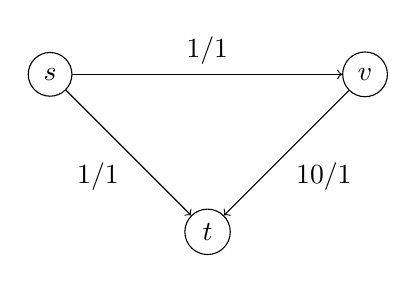
\begin{tikzpicture}
		\node[draw, circle] (S) at (0,2) {$s$};
		\node[draw, circle] (V) at (4,2) {$v$};
		\node[draw, circle] (T) at (2,0) {$t$};
		
		\path [->] (S) edge node[above] {$1/1$} (V);
		\path [->] (S) edge node[below left] {$1/1$} (T);
		\path [->] (V) edge node[below right] {$10/1$} (T);
		\end{tikzpicture}
		\caption{Ein Netzwerk mit Kantenbeschriftung $\tau_e / u_e$.}
		\label{figure-labels}
	\end{figure}
\end{remark}

Weiter kann man zeigen, dass man das $\alpha$ in Theorem~\ref{thm-alpha-extension-is-nash-flow} stets strikt positiv wählen kann:
\begin{proposition}
	Für einen dynamischen Nash-Fluss $f$ mit Zeithorizont $T$ und normierten schmalen Fluss $x'$ mit Knotenauslastungen $l'$ existiert ein $\alpha>0$, das sowohl (\ref{equation-alpha-queuing-edge}) und (\ref{equation-alpha-inactive-edge}) erfüllt.
	Dabei kann $\alpha$ gewählt werden zwischen $0$ und \[
	\inf\left(\left\{ \frac{q_{vw}(l_v(T))}{l_v' - l_w'} ~\middle|~ vw\in E_1, l_w' < l_v' \right\} \cup \left\{ \frac{l_v(T) + \tau_{vw} -l_w(T)}{l_w' - l_v'} ~\middle|~ vw\notin E_\theta, l_w' > l_v' \right\}\right).
	\]
\end{proposition}
\begin{proof}
	Für Kanten $vw$ mit positiver Warteschlange zur Zeit $T$ muss (\ref{equation-alpha-queuing-edge}), also $l_w(T) - l_v(T) + \alpha(l_w' - l_v') \geq \tau_{vw}$, gelten.
	Wegen Lemma~\ref{lemma-nash-flow-waiting-queue-implies-active-edge} ist dies äquivalent zu $\alpha(l_v' - l_w') \leq q_{vw}(l_v(T))$.
	Ist also $l_w'$ größer oder gleich $l_v'$, so ist die linke Seite nicht-positiv, sodass die Gleichung erfüllt ist.
	Für $l_w' < l_v'$ muss jedoch zusätzlich $\alpha\leq q_{vw}(l_v(T)) / (l_v' - l_w')$ gefordert werden.
	
	Für zur Zeit $\theta$ inaktive Kanten $vw$ muss~(\ref{equation-alpha-inactive-edge}), d.h. $\alpha(l_w' -l_v') \leq l_v(T) + \tau_{vw} - l_w(T)$, gelten.
	Per Definition ist $l_v(T) + \tau_{vw} - l_w(T)$ für inaktive Kanten positiv.
	Analog muss für diese Kanten mit $l_w' > l_v'$ also $\alpha \leq (l_v(T) + \tau_{vw} -l_w(T))/(l_w' - l_v')$ gefordert werden.
	
	Da alle diese oberen Schranken positiv sind, ist auch das Infimum $\alpha^*$ dieser Werte positiv.
\end{proof}

Dies hat Koch in~\cite{Koch2011} genutzt, um einen Algorithmus zur Berechnung von dynamischen Nash-Flüssen mit konstanter Netzwerkeinflussrate vorzuschlagen:
Ausgehend vom dynamischen Nullfluss mit Zeithorizont $0$ wird der Fluss nach und nach mit normierten schmalen Flüssen um einen möglichst großen Zeitraum $\alpha$ erweitert.

Ob dieser Algorithmus jedoch terminiert in dem Sinne, dass irgendwann ein $\alpha$ beliebig groß gewählt werden kann und somit der dynamische Nash-Fluss ab einem Zeitpunkt $T$ konstant gewählt werden kann, ist eine bisher unbeantwortete Frage.
Cominetti, Correa und Olver beantworten Teile der Frage in~\cite{CominettiExample}:
Übersteigt die minimale Warteschlangenkapazität $u(\delta^+(S))$ eines $s$-$t$-Schnitts $S$ den konstanten Netzwerkzufluss $d$ nicht, so erreicht ein dynamischer Nash-Fluss schließlich einen stabilen Zustand, ab dem der Fluss konstant ist.
Ob dieser Zustand jedoch durch endlich viele $\alpha$-Erweiterungen berechnet werden kann, bleibt ungeklärt.
Jedoch geben die Autoren ein Beispiel, in dem erst in der Größe des Graphen exponentiell viele $\alpha$-Erweiterungen zu einem stabilen Zustand führen.

Unter Benutzung des Lemmas von Zorn kann man jedoch die Existenz von dynamischen Nash-Flüssen mit konstantem Netzwerkzufluss zeigen:

\begin{theorem}
	Für einen konstanten Netzwerkzufluss $d\in\R_{> 0}$ existiert ein dynamischer Nash-Fluss.
\end{theorem}
\begin{proof}
	Man betrachte auf der Menge aller dynamischer Nash-Flüsse mit Zeithorizont $T$, wobei $T=\infty$ zugelassen wird, und Netzwerkzufluss $d$ die folgende Ordnung~$\preceq$:
	Für zwei dynamische Nash-Flüsse $f$ bzw. $g$ mit Zeithorizont $T^1$ bzw. $T^2$ gelte genau dann $(f, T^1)\preceq (g, T^2)$, wenn $T^1 \leq T^2$ gilt und $g^+_{vw}$ mit $f^+_{vw}$ bzw. $g^-_{vw}$ mit $f^-_{vw}$ auf $(-\infty, l_v(T^1)$ bzw. $(-\infty, l_w(T^1))$ für alle Kanten $vw$ übereinstimmen, wobei $l_v$ die früheste Ankunftszeit bzgl. $f$ an einem Knoten $v$ sein soll.
	Sei nun eine aufsteigende Kette $(f^i, T^i)_{i\in\N}$ bezüglich $\preceq$ gegeben.
	Man bemerke, dass für $i\leq j$ die frühesten Ankunftszeiten der Flüsse $f^i$ und $f^j$ auf $(-\infty, T^i)$ übereinstimmen.
	
	Man definiere nun $T^* \coloneq \lim_{i\in\N} T^i$ sowie die Ankunftszeit $l_v(\theta)$ an einem Knoten $v$ zur Zeit $\theta\in(-\infty, T^*)$, die von einem Fluss $f^i$ der Kette mit $T^i \geq \theta$ angenommen wird.
	Sei außerdem $l_v(T^*) \coloneq \lim_{i\in\N} l_v(T^i)$.
	Definiert man nun $f$ als den Fluss, dessen Zuflussrate $f_{vw}^+$ für $\theta<l_v(T^*)$ den Wert von $f^{i+}_{vw}(\theta)$ eines $i\in\N$ mit $l_v(T^i) > l_v(\theta)$ hat und für $\theta \geq l_v(T^*)$ den Wert $0$ hat, sowie dessen Abflussrate $f_{vw}^-$ für $\theta<l_w(T^*)$ den Wert von $f^{i-}_{vw}(\theta)$ eines $i\in\N$ mit $l_w(T^i) > l_w(\theta)$ hat und für $\theta \geq l_w(T^*)$ den Wert $0$ hat.
	Dann ist $f$ nicht nur ein zulässiger Fluss, sondern sogar ein dynamischer Nash-Fluss mit Zeithorizont $T^*$.
	Somit folgt, dass $(f, T^*)$ eine obere Schranke der Kette $(f^i, T^i)_{i\in\N}$ bezüglich $\preceq$ ist.
	Nach dem Lemma von Zorn besitzt die Ordnung $\preceq$ ein maximales Element $(f, T^*)$.
	Dann muss $T^*$ aber bereits unendlich sein, da man durch eine $\alpha$-Erweiterung von $f$ mit $\alpha > 0$ sonst einen dynamischen Nash-Fluss $(\tilde{f}, T^* + \alpha)$ erhält, für den $(\tilde{f}, T^* + \alpha) \npreceq (f, T^*)$ gelten würde.
\end{proof}

Mit der gleichen Argumentation kann man auch zeigen, dass auch für jeden rechts-konstanten Netzwerkzufluss ein dynamischer Nash-Fluss existiert:
Dabei muss lediglich $T^* + \alpha$ noch vor der nächsten Sprungstelle liegen.
Cominetti u. a. zeigen in \cite{Cominetti2015} sogar die Existenz für Netzwerke mit $\tau_e > 0$ für alle $e\in E$, bei denen der Netzwerkzufluss eine beliebige Funktion in $L^p(0,T)$ ist.